\newcommand{\loga}{logaritamske funkcije}
Logaritamska funkcija uzima broj i vraća potenciju na koju moramo stavitu bazu logaritamske funkcije kako bi dobili argument.
Pronalazimo je u obliku:
\[f(x) = log_ax\;a > 0,\; a \neq 1\]
\\
Logaritam s bazom \(e\) zovemo prirodni logaritam i označavamo ga \(\ln{x}\).
\subsubsection{Domena i kodomena \loga}
    Domena eksponencijalne funkcija je po definiciji skup \(\mathbb{R^+}\).
    To je intuitivno jasno jer ne možemo naći potenciju negativnog broja.
    Kodomena eksponencijalne funkcije skup \(\mathbb{R}\).

\subsubsection{Graf \loga}
    Specifičnost grafa eksponencijalne funkcije je da uvijek prolazi kroz točku \((0, 1)\).
    Mijenjamo li parametar \(a\), mijenja se \emph{"brzina"} rasta funkcije.
    Dodavanjem slobodnog koeficijnta mjenjanmo odsječak na y-osi.
    \begin{figure}[ht]
        \centering
        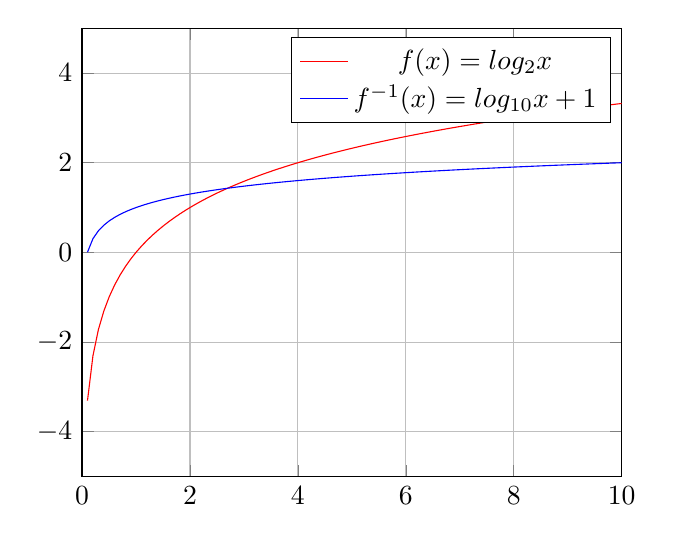
\begin{tikzpicture}
            \begin{axis}[
                grid=major,
                ymin=-5,
                ymax=5,
                xmin=0,
                xmax=10,
            ]
                \addplot[
                    color = red,
                    domain = 0:10,
                    samples = 100
                ]{log2(x)};
                \addlegendentry{\(f(x) = log_2x\)}
                \addplot[
                    color = blue,
                    domain = 0:10,
                    samples = 100
                ]{log10(x) + 1};
                \addlegendentry{\(f^{-1}(x) = log_{10}x + 1\)}
            \end{axis}
        \end{tikzpicture}
        \caption{Grafovi eksponencijalne funkcije s različitim parametrima}
        \label{fig:template}
    \end{figure}

\subsubsection{Nultočke i točke u kojima graf sječe y-os \loga}
    Nultočka logaritamske funkcije uvijek je (1, 0):
    \begin{equation*}
        \begin{split}
            0 &= log_ax \\
            x &= 1
        \end{split}
    \end{equation*}
    Njen graf ne sječe y-os.

\subsubsection{Parnost i neparnost \loga}
    Funkcija nije ni parna ni neparna jer ne zadovoljava definicije u \ref{par}.

\subsubsection{Periodičnost \loga}
    Funkcija nije periodična.

\subsubsection{Monotonost \loga}
    Funkcija je strogo rastuća.

\subsubsection{Omeđenost \loga}
    Funkcij
\subsubsection{Injektivnost i surjektivnost \loga}
\subsubsection{Inverz \loga}
Inverz eksponencijalne funkcije je logaritamska funkcija.
    \begin{figure}[ht]
        \centering
        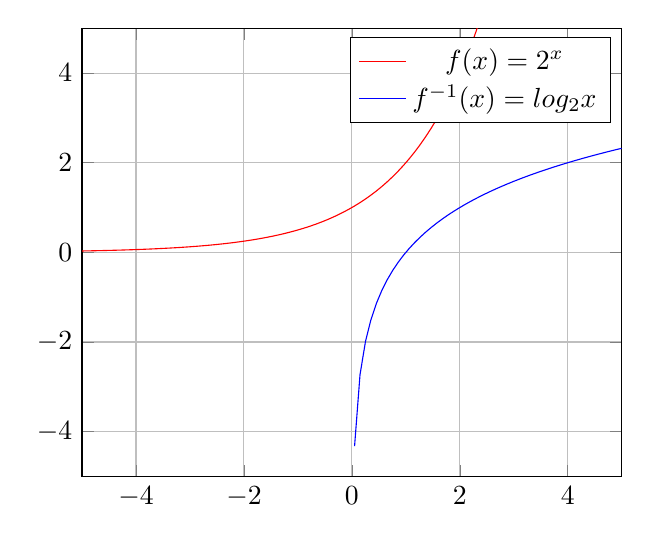
\begin{tikzpicture}
            \begin{axis}[
                grid=major,
                ymin=-5,
                ymax=5,
                xmin=-5,
                xmax=5,
            ]
                \addplot[
                    color = red,
                    samples = 100
                ]{2^x};
                \addlegendentry{\(f(x) = 2^x\)}
                \addplot[
                    color = blue,
                    samples = 100
                ]{log2(x)};
                \addlegendentry{\(f^{-1}(x) = log_2x\)}
            \end{axis}
        \end{tikzpicture}
        \caption{Grafovi funkcije i njenzinog inverzna}
        \label{fig:template}
    \end{figure}
    \\